\section{Subsistema: Controle}

\par O subsistema responsável pelo controle do carrinho autônomo controlará os motores (que a princípio estarão acoplados às rodinhas traseiras do carrinho). Além disso, esses subsistema fará a leitura dos sensores responsáveis por localizar o cadeirante e evitar colisões. 

\par Como mostrado na Figura \ref{fig:esqCarrinho}, os sensores se comunicarão com o microcontrolador, que por sua vez processará tais sinais elétricos e, com base em um algoritmo embarcado no próprio microcontrolador, acionará os atuadores (motores). Ademais, existirá um controle remoto que o usuário pode utilizar para efetuar as funções de liga/desliga. A Figura \ref{fig:esqCarrinho} exibe uma vista superior esquemática do protótipo a ser desenvolvido:

% \begin{figure}
% \centering
% \begin{minipage}{.5\textwidth}
%   \centering
%   
\includegraphics[width=.4\linewidth]{figuras/diagrama.png}
%   \captionof{figure}{Diagrama do sistema de controle do carrinho}
%   \label{fig:esqCarrinho}
% \end{minipage}%
% \begin{minipage}{.5\textwidth}
%   \centering
%   \includegraphics[width=.4\linewidth]{figuras/schematic.png}
%   \captionof{figure}{Vista superior esquemática do protótipo}
%   \label{fig:schematic}
% \end{minipage}
% \end{figure}

\begin{figure}[hb]
		\centering
		
\includegraphics[width=.5\textwidth]{figuras/diagrama.png}
		\caption{Esquemático do sistema de controle do carrinho}
		\label{fig:esqCarrinho}
\end{figure} 

\newpage 
\begin{figure}[hb]
		\centering
		\includegraphics[width=.5\textwidth]{figuras/schematic.png}
		\caption{Vista superior esquemática do protótipo}
		\label{fig:schematic}
\end{figure} 



\subsection{Relatório de Pesquisa Técnica}
\par O subsistema responsável pelo controle do carrinho autônomo, a princípio, pode ser dividido em três outros subsistemas:

\begin{itemize} 
\item Sistema de locomoção do carrinho;
\item Sistema de localização do cadeirante;
\item Sistema anti-colisão.
\end{itemize}

\subsubsection{Sistema de Locomoção do Carrinho}

    \par Inicialmente, pretende-se usar dois motores DC, de forma que cada um esteja acoplado à um roda traseira do carrinho. O controle desses motores será feito por meio da técnica PWM (\textit{Pulse Width Modulation}), que consiste em manter a frequência de uma onda quadrada fixa e variar o tempo que o sinal fica em nível lógico alto (\textit{duty cycle}), isto é, essa técnica proporciona o controle da velocidade de rotação do motor \cite{mecaweb}:
					
$$
Duty \hspace{0.1 cm} Cycle \propto Rotação \hspace{0.1  cm} do \hspace{0.1 cm} motor
$$

\par Os motores DC ou de corrente continua são muito utilizados nas áreas de robótica, mecatrônica e automação.  Eles funcionam quando uma tensão é aplicada em seus terminais de alimentação. O sentido que o motor gira depende do sentido de circulação da corrente em seus enrolamentos, ou seja, a mudança de polaridade da alimentação implica na mudança de direção de rotação. 

\par O controle do sentido de rotação de um motor DC pode ser feito usando um circuito eletrônico conhecido como Ponte-H. Elas são fundamentais no controle direcional do motor e permitem que um microcontrolador, que fornece sinais de corrente relativamente baixa, controle a velocidade dos motores que exigem correntes elevadas através de pinos de PWM. \cite{newtoncbraga}: 

\subsubsection{Sistema de Localização do Cadeirante}

\par Para o sistema de localização do cadeirante, foram consideradas três tecnologias diferentes:

\begin{itemize}  
\item Localização baseada em emissão/recepção de ondas eletromagnéticas;
\item Processamento de imagem;
\item Emissão de luz infravermelha.
\end{itemize}

\par O método de localização do cadeirante por meio de emissão/recepção de ondas eletromagnéticas analisado \cite{min2015active} consiste em um sistema em que o alvo emite ondas eletromagnéticas através de uma antena omnidirecional,  
e o carrinho autônomo conta com uma antena direcional que continuamente escaneia o ambiente à procura do sinal emitido pelo alvo. Um esquemático de tal sistema é apresentado na Figura \ref{fig:antenaElectroMagWave}. 

\newpage

\begin{figure}[ht]
		\centering
		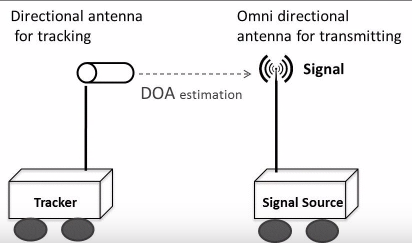
\includegraphics[width=.5\textwidth]{figuras/antenaElectroMagWave.png}
		\caption{Esquemático do sistema de controle do carrinho}
		\label{fig:antenaElectroMagWave}
	\end{figure} 
    
%{\color{red} traduzir a imagem e colocar fonte}

\par No sistema baseado em transmissão/recepção de ondas estudado, apenas uma antena direcional é empregada, de modo que a mesma varre o ambiente em ângulos obtusos de até 180$^{\circ}$. Uma desvantagem dessa implementação é que haveria um grande desgaste da estrutura mecânica que move a antena, uma vez que a estrutura que faz o escaneamento do ambiente se move de forma contínua durante todo o tempo de uso do protótipo. 

\par Estudou-se também um sistema baseado em processamento de imagem  \cite{isobe2014human} que consiste em detectar cores pré-determinadas, ou seja, o sistema é configurado de modo que uma determinada forma (com uma cor específica) seja isolado, e dessa forma, o sistema é capaz de identificar as mudanças de direção e distância do alvo através de detecção e análise das distorções nessa forma. É sabido, entretanto, que esse método de localização do alvo demanda uma ferramenta de maior poder de processamento. Sendo assim, microcontroladores mais simples como ATMega328, PIC32 e MSP430 não seriam as melhores opções para esse tipo de implementação.

\par Uma outra forma analisada de detectar a localização do cadeirante foi a desenvolvida por \cite{calcar} a qual emprega sensores infravermelhos de longo alcance para detectar a mudança de direção de um carrinho de controle remoto. Essa técnica, entretanto, requer que o alvo tenha uma superfície bem uniforme, em que as rajadas de luz infravermelha possam ser refletidas adequadamente. A Figura \ref{fig:IRbot} abaixo mostra como o sistema determinaria a condição de atuar sobre as rodas (se a diferença de distâncias lidas pelos sensores for maior que um determinado limiar $\epsilon$, então os atuadores são acionados e movem as rodas dianteiras).
\newpage
 
 \begin{figure}[ht]
		\centering
		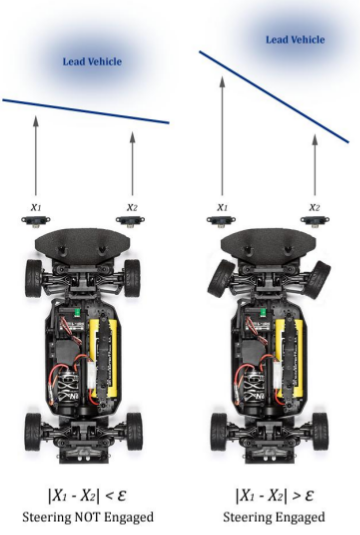
\includegraphics[width=.3\textwidth]{figuras/IRbot.png}
		\caption{Esquemático do sistema de controle do carrinho}
		\label{fig:IRbot}
	\end{figure} 

\par Após revisar e analisar os métodos supracitados, concluiu-se que, inicialmente a implementação do sistema de localização do cadeirante será abordada com uma combinação dos sistemas de detecção através de transmissão/recepção de ondas eletromagnéticas e de processamento de imagem. A estratégia é trabalhar com as duas frentes de forma paralela e ao fim, se possível, integrar as duas em um mesmo produto final. Caso não seja possível entregar as duas soluções integradas, espera-se que ao menos uma delas esteja completamente funcional e atendendo todos os requisitos funcionais e não funcionais do projeto. 

\subsubsection{Sistema de Anti-Colisão}
\par Esse sistema tem como principais objetivos:

\begin{itemize}
\item Manter uma determinada distância entre o usuário (cadeirante) e o carrinho,
\item Evitar as colisões com os objetos presentes no ambiente do supermercado
\end{itemize}

\par Tal sistema consistirá em um conjunto de sensores ultrassônicos os quais efetuam leituras de distâncias de 2 cm a 4 m com precisão de até 3 mm. O posicionamento de tais sensores será feito de uma forma em que seja possível  \cite{flipeflop}.

\subsection{Algoritmos}

\par Para a boa realização do projeto será necessário a integração de vários algoritmos específicos de cada problema encontrado. A partir de pesquisas preliminares chegamos a alguns possíveis candidatos a aplicação na solução final. Seguindo o fluxo do diagrama da Figura \ref{fig:diagramaAlg} é possível visualizar os principais blocos de processamento e quais algoritmos serão necessários para realização de cada etapa.

\begin{figure}[ht]
	\centering
	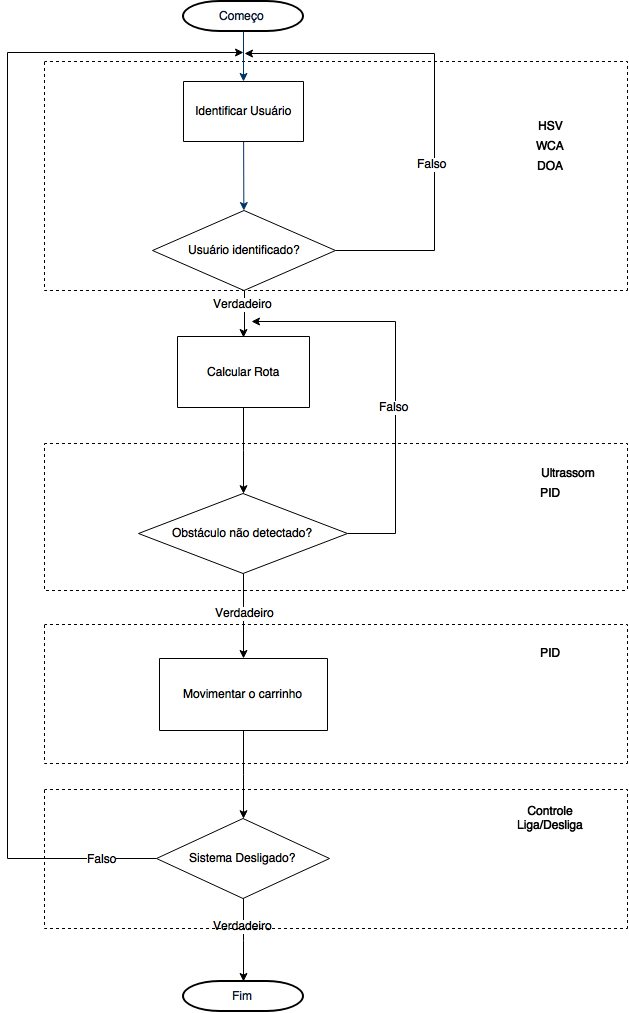
\includegraphics[width=.7\textwidth]{figuras/DiagramaAlgoritimos.png}
	\caption{Diagrama de blocos, fluxo dos algoritmos. Fonte: Autores}
	\label{fig:diagramaAlg}
\end{figure} 
    
\subsubsection{Controlador de posicionamento}

\par O módulo controlador de posicionamento será necessário para tratar e interpretar o sinal dos sensores de detecção de obstáculos e identificação do usuário. A partir disso poderá tomar decisões lógicas para determinar o caminho e a velocidade do carrinho de compras. Para tal, será necessário o uso de algoritmos como:

\subsubsubsection{Controlador PID} 

	\par PID é uma abreviação para "Proporcional, Integral, Derivativo" (\textit{Proportional, Integral, Derivative} em tradução livre), que em termos simples, é um controlador que visa minimizar os erros ao longo do tempo através de ajustes, e para realizar essa tarefa utiliza de um mecanismo de \textit{feedback} em \textit{loop} para reajustar a variável $u(t)$, segundo a fórmula abaixo: 

$$
u(t)=K_p e(t)+K_i\int_0^t e(t) dt + K_d\frac{de(t)}{dt}
$$

Tendo isso como base, podemos controlar a aceleração dos motores a serem usados no carrinho e corrigir os erros de posicionamento produzidos pelos sensores. Já que esse controlador é versátil e necessita de poucas mudanças em sua modelagem para ser aplicável em outro contexto. \cite{wescott2000}

\subsubsection{Detecção do usuário}

\subsubsubsection{WCA e DOA}

\par Diante de estudo realizado sobre como detectar e reconhecer sinais eletromagnéticos, constatou-se que será necessário o uso de algoritmos como WCA (\textit{Weighted Centroid Algorithm}, em inglês) e DOA (\textit{Direction of Arrival}, em inglês) para determinar a localização e a direção do usuário \cite{min2015active}. 

Através do estudo de artigos científicos coletados em bases reconhecidas - como o \textit{IEEExplorer}, \textit{Scopus}, \textit{Springer} e \textit{Science Direct} -, foi possível concluir que tais tecnologias dependerão de grande esforço de estudo para que sejam aplicadas ao presente trabalho. Para a Fase 3 do projeto, este estudo sera de fundamental importância.

\subsubsubsection{Processamento de imagens}

	Um dos principais desafios do projeto é fazer com que o carrinho ao seguir o cadeirante seja capaz de reagir ao ambiente, antecipar um obstáculo ou evitar uma colisão, ou seja ele deve se movimentar de forma autônoma. 
Para que a movimentação autônoma seja possível, uma grande parte dos veículos deste tipo empregam algoritmos de processamento de imagem bem como sensores para permitir identificar o ambiente no qual o veículo está se movimentando. Para lidar com todas essas informações é necessário utilizar programas altamente eficientes e robustos, em muitos casos utilizando \textit{frameworks} desenvolvidas especialmente para aplicações de processamento de imagens e processamento de sinais.
	
    Para a programação dos algoritmos do presente trabalho, depois de realizada diversas pesquisas cogita-se utilizar uma biblioteca \textit{open source}, robusta e popular conhecida como \textit{OpenCV}. Esta escolha deve-se ao fato de ela contar com uma ampla gama de funções que vão desde interface com o usuário e com câmeras, algoritmos de processamento de imagem, até elementos de inteligência artificial. A biblioteca não está vinculada a nenhum hardware específico o que possibilita a escolha independente dos materiais a serem utilizados. Seu foco principal está exatamente nas aplicações em tempo real, o que a torna bastante interessante para aplicações de visão robótica.
	
    Existem milhares de algoritmos para processamento de imagens , muitos deles são bastante avançados. Entretanto para este projeto, deseja-se implementar um dos mais simples esquemas: rastreamento de cor. Este tipo de algoritmo de acompanhamento de cor está preocupado apenas com os dados de cor. Nenhuma análise complexa da imagem é necessário. O algoritmo não diferencia entre tons de cor ou objetos separados, com a mesma cor. Ele simplesmente relata que partes da imagem estão acima de um limite de cor e quais partes não estão.
	
    Sendo assim, planeja-se que o robô se mova para a frente quando a cor é concentrada no centro da tela, ou cobre a tela. Se desloque para a esquerda quando a cor é concentrada na metade esquerda da tela e se mova para a direita quando a cor está concentrada no lado direito. 
	
    Poderíamos certamente fazer controles de movimento mais detalhadas, no entanto, optou-se por fazer o mais simples possível para garantir que o projeto seja entregue dentro do prazo. 
	
    Para finalizar, será explicando de maneira breve como será trabalhada a parte de processamento de imagens. O trabalho será desenvolvido utilizando a biblioteca OpenCV integrada ao Ambiente de Desenvolvimento da \textit{Microsoft, Visual Studio 2012} na linguagem C++, ou no sistema Linux. 
	
   A aquisição das imagens do vídeo processado será realizada por meio da função do \textit{OpenCV}, \textit{cvCapture}, e como esta captura uma imagem em RGB, será necessária a conversão da mesma para o espaço de cores HSV, utilizando a função \textit{cvtColor}. Logo após faremos uma (limiarização) multinível. Para que a detecção do objeto seja mais precisa será necessária a aplicação de filtros morfológicos. Logo após esse processo obteremos o objeto selecionado na imagem em tempo real, e para tal utilizaremos o centro obtido por meio dos \textit{Moments}, definidos na \textit{OpenCV}.
 
\subsection{Riscos associados}

Para um bom desenvolvimento do projeto, devem-se levar em conta fatores que possam atrapalhar esse processo, os  riscos associados. Entre eles estão:

\begin{itemize}
\item Alimentação insuficiente do hardware;
\item Não conseguir atender o prazo de entrega do subsistema;
\item Bugs não encontrados no algoritmo;
\item Falha/queima de componentes;
\item Falta de conhecimento para desenvolver o produto;
\item Falha do computador;
\item Serviço de hospedagem do repositório git fechar;
\item Problema de saúde ou desistência de integrante;
\item Software de produção ou sistema falhar.
\end{itemize}

\subsection{Cronograma Físico-Financeiro}
Para o projeto do subsistema Controle e Automação, foi feita uma estimativa de tempo de aquisição e preços possíveis dos componentes desse subproduto.

% ######## init table ########
\begin{table}[h]
 \centering
% distancia entre a linha e o texto
 {\renewcommand\arraystretch{1.25}
 \caption{Cronograma custo-financeiro Controle.}
 \begin{tabular}{ l l l }
  \cline{1-1}\cline{2-2}\cline{3-3}  
    \multicolumn{1}{|c|}{\textbf{Componentes/Recursos} \centering } &
    \multicolumn{1}{c|}{\textbf{Data de aquisição} \centering } &
    \multicolumn{1}{c|}{\textbf{Estimativa de preço} \centering }
  \\  
  \cline{1-1}\cline{2-2}\cline{3-3}  
    \multicolumn{1}{|p{3.850cm}|}{Microprocessador (CPU) \centering } &
    \multicolumn{1}{p{4.217cm}|}{14/09 a 4/10/2016 \centering } &
    \multicolumn{1}{p{4.217cm}|}{R\$ 25,00 \centering }
  \\  
  \cline{1-1}\cline{2-2}\cline{3-3}  
    \multicolumn{1}{|p{3.850cm}|}{Sensores \centering } &
    \multicolumn{1}{p{4.217cm}|}{14/09 a 4/10/2016 \centering } &
    \multicolumn{1}{p{4.217cm}|}{R\$ 30,00 \centering }
  \\  
  \cline{1-1}\cline{2-2}\cline{3-3}  
    \multicolumn{1}{|p{3.850cm}|}{Ponte h \centering } &
    \multicolumn{1}{p{4.217cm}|}{14/09 a 4/10/2016 \centering } &
    \multicolumn{1}{p{4.217cm}|}{R\$ 50,00 \centering }
  \\  
  \cline{1-1}\cline{2-2}\cline{3-3}  
    \multicolumn{1}{|p{3.850cm}|}{Raspberry Pi  \centering } &
    \multicolumn{1}{p{4.217cm}|}{14/09 a 4/10/2016 \centering } &
    \multicolumn{1}{p{4.217cm}|}{R\$ 300.00 \centering }
  \\  
  \cline{1-1}\cline{2-2}\cline{3-3}  
    \multicolumn{1}{|p{3.850cm}|}{Codificador e Decofificador RF \centering } &
    \multicolumn{1}{p{4.217cm}|}{14/09 a 4/10/2016 \centering } &
    \multicolumn{1}{p{4.217cm}|}{R\$ 40,00 \centering }
  \\  
  \cline{1-1}\cline{2-2}\cline{3-3}  
    \multicolumn{1}{|p{3.850cm}|}{Antena \centering } &
    \multicolumn{1}{p{4.217cm}|}{14/09 a 4/10/2016 \centering } &
    \multicolumn{1}{p{4.217cm}|}{R\$ 150,00 \centering }
  \\  
  \cline{1-1}\cline{2-2}\cline{3-3}  
    \multicolumn{1}{|p{3.850cm}|}{Câmera (Raspberry) \centering } &
    \multicolumn{1}{p{4.217cm}|}{14/09 a 4/10/2016 \centering } &
    \multicolumn{1}{p{4.217cm}|}{R\$ 70,00 \centering }
  \\  
  \cline{1-1}\cline{2-2}\cline{3-3}  
    \multicolumn{2}{|p{3.850cm}|}{Total \centering } &
    \multicolumn{1}{p{4.217cm}|}{R\$ 665,00 \centering }
  \\  
  \hline

 \end{tabular} }
\end{table}


\subsection{Cronograma de atividades}

A Tabela \ref{tab:cronograma_controle} apresenta todas as atividades que serão realizadas pelo subgrupo de controle até a entrega final do produto.

% ######## init table ########
\begin{table}[!htbp]
 \centering
 \caption{Cronograma de atividades do Subsistema Controle} \label{tab:cronograma_controle}
% distancia entre a linha e o texto
 {\renewcommand\arraystretch{1.25}
 \begin{tabular}{ l l l l l }
  \cline{1-1}\cline{2-2}\cline{3-3}\cline{4-4}\cline{5-5}  
    \multicolumn{1}{|p{6.900cm}|}{\textbf{Atividades}} &
    \multicolumn{1}{p{1.817cm}|}{\textbf{Duração}} &
    \multicolumn{1}{p{1.650cm}|}{\textbf{Data de início}} &
    \multicolumn{1}{p{1.550cm}|}{\textbf{Data de fim}} &
    \multicolumn{1}{p{2.000cm}|}{\textbf{Status}}
  \\  
  \cline{1-1}\cline{2-2}\cline{3-3}\cline{4-4}\cline{5-5}  
    \multicolumn{1}{|p{6.900cm}|}{\textbf{Fase 1}} &
    \multicolumn{1}{p{1.817cm}|}{\textbf{7 dias}} &
    \multicolumn{1}{p{1.650cm}|}{\textbf{17/08}} &
    \multicolumn{1}{p{1.550cm}|}{\textbf{24/08}} &
    \multicolumn{1}{p{2.000cm}|}{\textbf{Realizado}}
  \\  
  \cline{1-1}\cline{2-2}\cline{3-3}\cline{4-4}\cline{5-5}  
    \multicolumn{1}{|p{6.900cm}|}{Pesquisar trabalhos correlatos} &
    \multicolumn{1}{p{1.817cm}|}{5 dias} &
    \multicolumn{1}{p{1.650cm}|}{19/08} &
    \multicolumn{1}{p{1.550cm}|}{24/08} &
    \multicolumn{1}{p{2.000cm}|}{Realizado}
  \\  
  \cline{1-1}\cline{2-2}\cline{3-3}\cline{4-4}\cline{5-5}  
    \multicolumn{1}{|p{6.900cm}|}{Definir cronograma de controle} &
    \multicolumn{1}{p{1.817cm}|}{1 dia} &
    \multicolumn{1}{p{1.650cm}|}{24/8} &
    \multicolumn{1}{p{1.550cm}|}{24/8} &
    \multicolumn{1}{p{2.000cm}|}{Realizado}
  \\  
  \cline{1-1}\cline{2-2}\cline{3-3}\cline{4-4}\cline{5-5}  
    \multicolumn{1}{|p{6.900cm}|}{\textbf{Fase 2}} &
    \multicolumn{1}{p{1.817cm}|}{\textbf{15 dias}} &
    \multicolumn{1}{p{1.650cm}|}{\textbf{24/8}} &
    \multicolumn{1}{p{1.550cm}|}{\textbf{9/9}} &
    \multicolumn{1}{p{2.000cm}|}{Realizado}
  \\  
  \cline{1-1}\cline{2-2}\cline{3-3}\cline{4-4}\cline{5-5}  
    \multicolumn{1}{|p{6.900cm}|}{Propor um esquema de solução} &
    \multicolumn{1}{p{1.817cm}|}{1 dia} &
    \multicolumn{1}{p{1.650cm}|}{24/8} &
    \multicolumn{1}{p{1.550cm}|}{24/8} &
    \multicolumn{1}{p{2.000cm}|}{Realizado}
  \\  
  \cline{1-1}\cline{2-2}\cline{3-3}\cline{4-4}\cline{5-5}  
    \multicolumn{1}{|p{6.900cm}|}{Pesquisar componentes do esquema  			

Sensores e processadores – eletrônica  			

Algoritmos - software} &
    \multicolumn{1}{p{1.817cm}|}{2 dias} &
    \multicolumn{1}{p{1.650cm}|}{24/08} &
    \multicolumn{1}{p{1.550cm}|}{26/8} &
    \multicolumn{1}{p{2.000cm}|}{Realizado}
  \\  
  \cline{1-1}\cline{2-2}\cline{3-3}\cline{4-4}\cline{5-5}  
    \multicolumn{1}{|p{6.900cm}|}{Projetar montagem e fabricação} &
    \multicolumn{1}{p{1.817cm}|}{1 dia} &
    \multicolumn{1}{p{1.650cm}|}{31/8} &
    \multicolumn{1}{p{1.550cm}|}{31/8} &
    \multicolumn{1}{p{2.000cm}|}{Realizado}
  \\  
  \cline{1-1}\cline{2-2}\cline{3-3}\cline{4-4}\cline{5-5}  
    \multicolumn{1}{|p{6.900cm}|}{Escrever relatório} &
    \multicolumn{1}{p{1.817cm}|}{3 dias} &
    \multicolumn{1}{p{1.650cm}|}{31/8} &
    \multicolumn{1}{p{1.550cm}|}{2/9} &
    \multicolumn{1}{p{2.000cm}|}{Realizado}
  \\  
  \cline{1-1}\cline{2-2}\cline{3-3}\cline{4-4}\cline{5-5}  
    \multicolumn{1}{|p{6.900cm}|}{Apresentação - todos} &
    \multicolumn{1}{p{1.817cm}|}{1 dia} &
    \multicolumn{1}{p{1.650cm}|}{9/9} &
    \multicolumn{1}{p{1.550cm}|}{9/9} &
    \multicolumn{1}{p{2.000cm}|}{Realizado}
  \\  
  \cline{1-1}\cline{2-2}\cline{3-3}\cline{4-4}\cline{5-5}  
    \multicolumn{1}{|p{6.900cm}|}{\textbf{Fase 3}} &
    \multicolumn{1}{p{1.817cm}|}{\textbf{61 dias}} &
    \multicolumn{1}{p{1.650cm}|}{\textbf{9/9}} &
    \multicolumn{1}{p{1.550cm}|}{\textbf{9/11}} &
    \multicolumn{1}{p{2.000cm}|}{\textbf{À fazer}}
  \\  
  \cline{1-1}\cline{2-2}\cline{3-3}\cline{4-4}\cline{5-5}  
    \multicolumn{1}{|p{6.900cm}|}{Definir e escolher componentes a - eletrônica} &
    \multicolumn{1}{p{1.817cm}|}{6 dias} &
    \multicolumn{1}{p{1.650cm}|}{14/9} &
    \multicolumn{1}{p{1.550cm}|}{20/9} &
    \multicolumn{1}{p{2.000cm}|}{À fazer}
  \\  
  \cline{1-1}\cline{2-2}\cline{3-3}\cline{4-4}\cline{5-5}  
    \multicolumn{1}{|p{6.900cm}|}{Definir algoritmos utilizados – software} &
    \multicolumn{1}{p{1.817cm}|}{6 dias} &
    \multicolumn{1}{p{1.650cm}|}{14/9} &
    \multicolumn{1}{p{1.550cm}|}{20/9} &
    \multicolumn{1}{p{2.000cm}|}{À fazer}
  \\  
  \cline{1-1}\cline{2-2}\cline{3-3}\cline{4-4}\cline{5-5}  
    \multicolumn{1}{|p{6.900cm}|}{Realizar simulações das placas projetadas – eletrônica} &
    \multicolumn{1}{p{1.817cm}|}{3 dias} &
    \multicolumn{1}{p{1.650cm}|}{20/9} &
    \multicolumn{1}{p{1.550cm}|}{23/9} &
    \multicolumn{1}{p{2.000cm}|}{À fazer}
  \\  
  \cline{1-1}\cline{2-2}\cline{3-3}\cline{4-4}\cline{5-5}  
    \multicolumn{1}{|p{6.900cm}|}{Testar de algoritmo em primeiro protótipo – software} &
    \multicolumn{1}{p{1.817cm}|}{30 dias} &
    \multicolumn{1}{p{1.650cm}|}{23/9} &
    \multicolumn{1}{p{1.550cm}|}{21/10} &
    \multicolumn{1}{p{2.000cm}|}{À fazer}
  \\  
  \cline{1-1}\cline{2-2}\cline{3-3}\cline{4-4}\cline{5-5}  
    \multicolumn{1}{|p{6.900cm}|}{Confeccionar placas – eletrônica} &
    \multicolumn{1}{p{1.817cm}|}{16 dias} &
    \multicolumn{1}{p{1.650cm}|}{4 /10} &
    \multicolumn{1}{p{1.550cm}|}{21/10} &
    \multicolumn{1}{p{2.000cm}|}{À fazer}
  \\  
  \cline{1-1}\cline{2-2}\cline{3-3}\cline{4-4}\cline{5-5}  
    \multicolumn{1}{|p{6.900cm}|}{Testar placas – eletrônica} &
    \multicolumn{1}{p{1.817cm}|}{3 dias} &
    \multicolumn{1}{p{1.650cm}|}{25/10} &
    \multicolumn{1}{p{1.550cm}|}{28/10} &
    \multicolumn{1}{p{2.000cm}|}{À fazer}
  \\  
  \cline{1-1}\cline{2-2}\cline{3-3}\cline{4-4}\cline{5-5}  
    \multicolumn{1}{|p{6.900cm}|}{Projetar a integração com outros subsistemas - todos} &
    \multicolumn{1}{p{1.817cm}|}{3 dias} &
    \multicolumn{1}{p{1.650cm}|}{25/10} &
    \multicolumn{1}{p{1.550cm}|}{28/10} &
    \multicolumn{1}{p{2.000cm}|}{À fazer}
  \\  
  \cline{1-1}\cline{2-2}\cline{3-3}\cline{4-4}\cline{5-5}  
    \multicolumn{1}{|p{6.900cm}|}{Documentar avanços} &
    \multicolumn{1}{p{1.817cm}|}{2 dias} &
    \multicolumn{1}{p{1.650cm}|}{2/11} &
    \multicolumn{1}{p{1.550cm}|}{4/11} &
    \multicolumn{1}{p{2.000cm}|}{À fazer}
  \\  
  \cline{1-1}\cline{2-2}\cline{3-3}\cline{4-4}\cline{5-5}  
    \multicolumn{1}{|p{6.900cm}|}{Apresentação – todos} &
    \multicolumn{1}{p{1.817cm}|}{1 dia} &
    \multicolumn{1}{p{1.650cm}|}{9/11} &
    \multicolumn{1}{p{1.550cm}|}{9/11} &
    \multicolumn{1}{p{2.000cm}|}{À fazer}
  \\  
  \cline{1-1}\cline{2-2}\cline{3-3}\cline{4-4}\cline{5-5}  
    \multicolumn{1}{|p{6.900cm}|}{\textbf{Fase 4}} &
    \multicolumn{1}{p{1.817cm}|}{\textbf{23 dias}} &
    \multicolumn{1}{p{1.650cm}|}{\textbf{9/11}} &
    \multicolumn{1}{p{1.550cm}|}{\textbf{2/12}} &
    \multicolumn{1}{p{2.000cm}|}{À fazer}
  \\  
  \cline{1-1}\cline{2-2}\cline{3-3}\cline{4-4}\cline{5-5}  
    \multicolumn{1}{|p{6.900cm}|}{Testar a integração com os subsistemas} &
    \multicolumn{1}{p{1.817cm}|}{12 dias} &
    \multicolumn{1}{p{1.650cm}|}{11/11} &
    \multicolumn{1}{p{1.550cm}|}{23/11} &
    \multicolumn{1}{p{2.000cm}|}{À fazer}
  \\  
  \cline{1-1}\cline{2-2}\cline{3-3}\cline{4-4}\cline{5-5}  
    \multicolumn{1}{|p{6.900cm}|}{Definir o protótipo final} &
    \multicolumn{1}{p{1.817cm}|}{5 dias} &
    \multicolumn{1}{p{1.650cm}|}{25/11} &
    \multicolumn{1}{p{1.550cm}|}{30/11} &
    \multicolumn{1}{p{2.000cm}|}{À fazer}
  \\  
  \cline{1-1}\cline{2-2}\cline{3-3}\cline{4-4}\cline{5-5}  
    \multicolumn{1}{|p{6.900cm}|}{Documentar avanços finais} &
    \multicolumn{1}{p{1.817cm}|}{5 dias} &
    \multicolumn{1}{p{1.650cm}|}{25/11} &
    \multicolumn{1}{p{1.550cm}|}{30/11} &
    \multicolumn{1}{p{2.000cm}|}{À fazer}
  \\  
  \cline{1-1}\cline{2-2}\cline{3-3}\cline{4-4}\cline{5-5}  
    \multicolumn{1}{|p{6.900cm}|}{Apresentação final} &
    \multicolumn{1}{p{1.817cm}|}{1 dia} &
    \multicolumn{1}{p{1.650cm}|}{2/12} &
    \multicolumn{1}{p{1.550cm}|}{2/12} &
    \multicolumn{1}{p{2.000cm}|}{À fazer}
  \\  
  \hline

 \end{tabular} }
\end{table}

			
\newpage


